
\section{Описание экспериментальной установки BM@N}

\subsection{Ускорительный комплекс NUCLOTRON-NICA}

Эксперимент BM@N располагается на выведенном пучке ускорителя NUCLOTRON, который является частью ускорительного комплеса NICA, ОИЯИ, Дубна.
Линейный ускоритель тяжелых ионов Linac инжектирует пучок в кольцевой ускоритель Boster.
После ускорения тяжелых ионов в кольце Booster до энергии в $0.5A$~ГэВ, пучок подаётся на NUCLOTRON.
Максимальные энергии, достижимые Nuclotron составляют до $4.5A$~ГэВ.
После ускорения ядер до необходимой энергии, пучок может быть отправлен как на эксперимент BM@N, так и на коллайдер NICA.

\subsection{Схема установки}

BM@N является экспериментом с фиксированной мишенью.
Схема экспериментальной установке представлена на рис.~\ref{fig:bmn_layout}.
%
\begin{figure}[ht]
\begin{center}
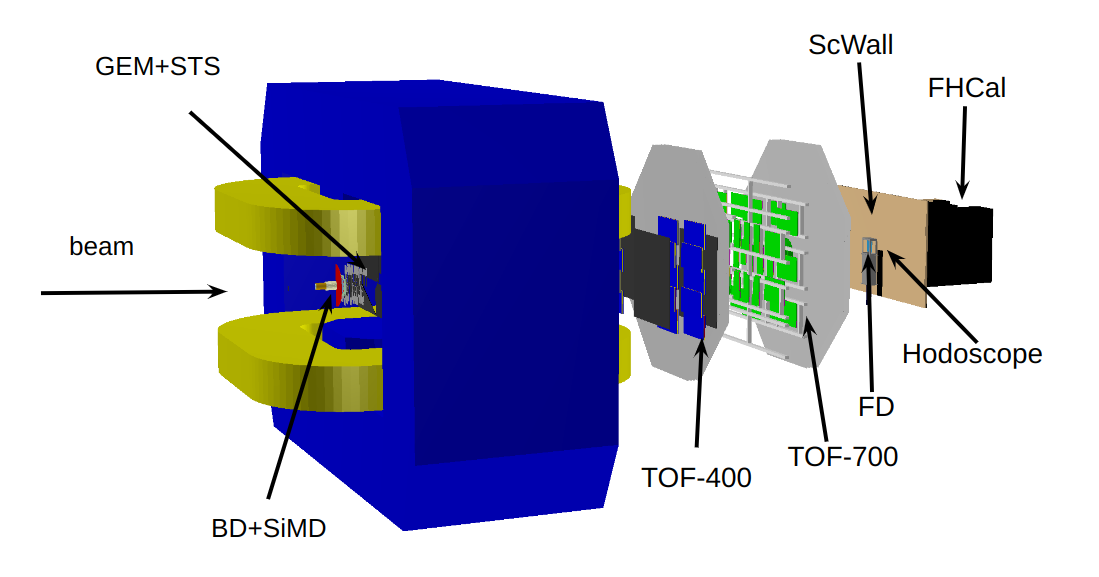
\includegraphics[width=0.95\linewidth]{images/BM@N_layout.png}
\caption{Схема эксперимента BM@N.}
\label{fig:bmn_layout}
\end{center}
\end{figure}

\subsection{Трекинговая система}

Система реконструкции траекторий заряженных частиц в эксперименте BM@N состоит из четырех станций кремниевых детекторов (Silicon) и семи станций газо-электронных умножителей (GEM). 
В отличие от HADES, трекинговая система целиком находится в магнитном поле дипольного магнита что позволяет с большой точностью восстанавливать импульсы рожденных в столкновении заряженных частиц.
На рис.~\ref{fig:bmn_tracking} представлено схематическое изображение трекинговой системы в эксперименте BM@N.
Траектории заряженных частиц отклоняются магнитным полем дипольного магнита, что позволяет восстанавливать импульс заряженных частиц.
Вакуумная пучковая труба позволяет минимизировать столкновения ядер цезия с атомами азота, кислорода и прочими примесями.
Поскольку вакуумная труба также расположена в магнитном поле, она имеет искривлённую форму для свободного прохождения невзаимодействоваших ядер пучка.  
%
\begin{figure}[ht]
\begin{center}
    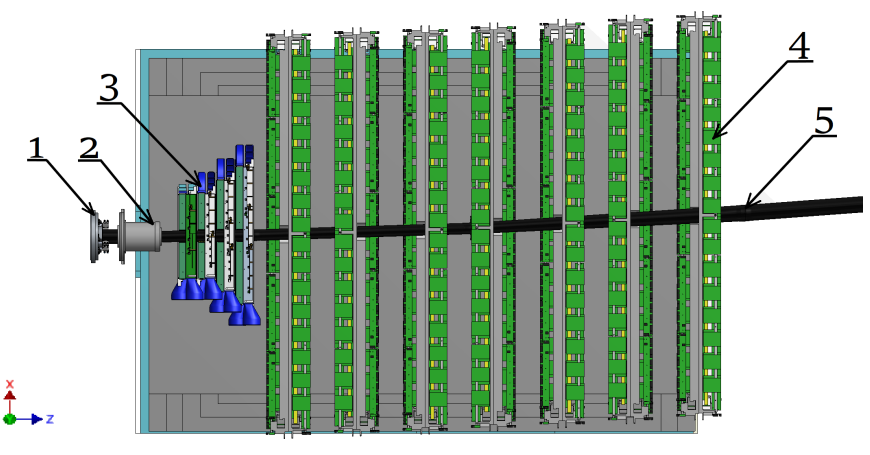
\includegraphics[width=0.75\linewidth]{images/bmn_tracking_system.png}
    \caption{Схематическое изображение трекинговой системы в эксперименте BM@N. Цифрами (1) обозначена мишень,
    (2) --- Barell Detector, (3) --- STS, (4) --- GEM, (5) --- Beam Pipe }
    \label{fig:bmn_tracking}
\end{center}
\end{figure}


\subsection{Времяпролётные детекторы TOF-400 и TOF-700}

В эксперименте BM@N идентификация заряженных частиц может выполняться только времяпролётным методом, используя информацию с двух станций времяпролётных детекторов, расположенных на расстоянии 400 и 700~см от мишении (TOF-400 и TOF-700 соответственно).
Подсистема TOF-400 состоит из двух половин, размещенных симметрично относительно оси пучка.
Каждая половина собрана из 5 MRPC детекторов.
Каждый детектор покрывает площадь $60\times30$~см$^2$.
Полный геометрический аксептанс всей сборки равен $1.1\times1.3$~м$^2$.
Дектор TOF-700 покрывает площадь в $3.2\time2.2$~м$^2$.
Подсистема также собрана из MRPC детекторов.

На рис.~\ref{fig:bmn_beta_pq} показано распределение заряженных частиц по относительной скорости $\beta=v/c$ и импульсу деленному на заряд $p/q$.
%
\begin{figure}[ht]
\begin{center}
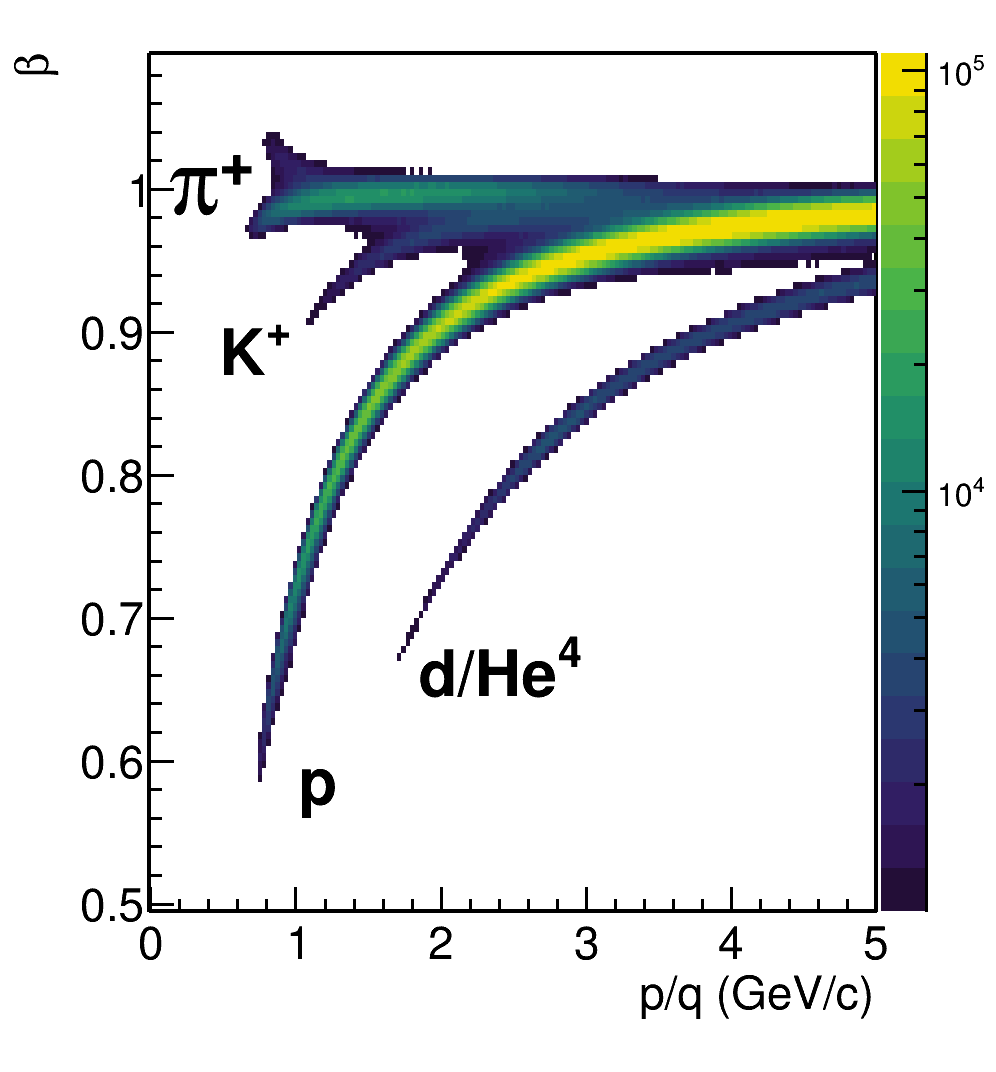
\includegraphics[width=0.55\linewidth]{images/beta_pq.png}
\caption{Распределение заряженных частиц по относительной скорости $\beta=v/c$ и импульсу деленному на заряд $p/q$.}
\label{fig:bmn_beta_pq}
\end{center}
\end{figure}

\subsection{Передний адронный калориметр FHCal}

В эксперименте BM@N энерговыделение спектаторных фрагментов измеряется при помощи переднего адронного калориметра FHCal.
Адронный калориметр состоит из 54 модулей, их размеры --- $15\times15$ и $20\times20$~см.
Схема расположения модулей калориметра представлена на рис.~\ref{fig:fhcal_layout} справа.
Большие модули ($20\times20$~см) обозначены желтым цветом, малые модули ($15\times15$) обозначены синим цветом. 
%
\begin{figure}[ht]
\begin{center}
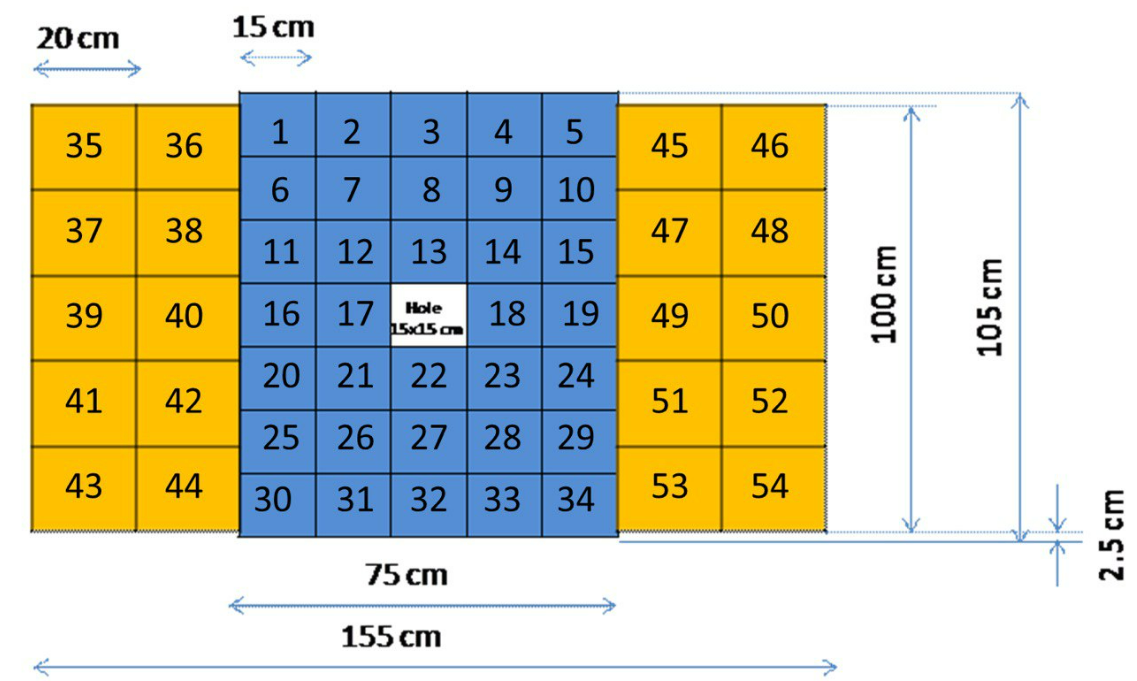
\includegraphics[width=0.55\linewidth]{images/FHCal_modules.png}
\caption{Схема расположения модулей переднего адронного калориметра FHCal.}
\label{fig:fhcal_layout}
\end{center}
\end{figure}

\section{Выводы к главе 2}

В главе описывается устройство экспериментальной установки HADES. 
Рассмотрены принципы работы основных детекторных подсистем, таких как трекинговая система, триггерная система, времяпролётная система и передний годоскоп Forward Wall.
В главе приведено краткое описание установки BM@N и ее детекторов.
Рассмотрены принципы работы трекинговой системы, описано устройство времяпролётной системы и переднего адронного калориметра FHCal.
